\documentclass[11pt]{article}

\usepackage[margin=1in]{geometry}
\usepackage[T1]{fontenc}
\usepackage{lmodern}
\usepackage{microtype}
\usepackage{xcolor}
\usepackage{hyperref}
\usepackage{listings}
\usepackage{tikz}
\usetikzlibrary{arrows.meta,positioning,shapes.geometric}

\hypersetup{
  colorlinks=true,
  linkcolor=blue!60!black,
  urlcolor=blue!60!black
}

\lstdefinelanguage{CDSTR}{
  morekeywords={system,vars,vars*,domain,domain*,init,action,next,invariant,property,
    defn,defmacro,include,load-java-enums,load-proto-enums,quote,set,not,eventually,if,then,assign,to,as,equals,
    unchanged*,forall,exists,and,or,alternate-scenarios,implies,in,let,list,fn,map},
  sensitive=true,
  morecomment=[l]{;},
  morestring=[b]"
}

\lstset{
  basicstyle=\ttfamily\small,
  keywordstyle=\color{blue!65!black}\bfseries,
  commentstyle=\color{green!35!black},
  stringstyle=\color{red!55!black},
  showstringspaces=false,
  columns=fullflexible,
  keepspaces=true,
  frame=single,
  breaklines=true
}

\title{CDSTR Reference Manual\\\large Clojure Front End, Shell, and Tooling}
\author{Sambuddha Majumder and Jayanta Majumder}
\date{\today}

\begin{document}
\maketitle
\tableofcontents

\section{Purpose and Scope}

CDSTR is the Clojure-shaped front end for \texttt{dstr}.  It reads
\texttt{.cdstr} files, macroexpands their DSL forms with Clojure, and emits the
same normalized JSON format used by the core checker and graph tools.  The
front end lives in the standalone \texttt{clj-dstr} Java project and can be run
with Maven or Gradle.  Clojure is obtained from Maven repositories, so no
separate Clojure installation is required beyond the Java build tool.

CDSTR is useful when a model benefits from homoiconicity and Clojure macros but
should still target the same explicit-state JSON as DSTR and TDSTR.

\section{Tooling Layout}

\begin{center}
\resizebox{\textwidth}{!}{%
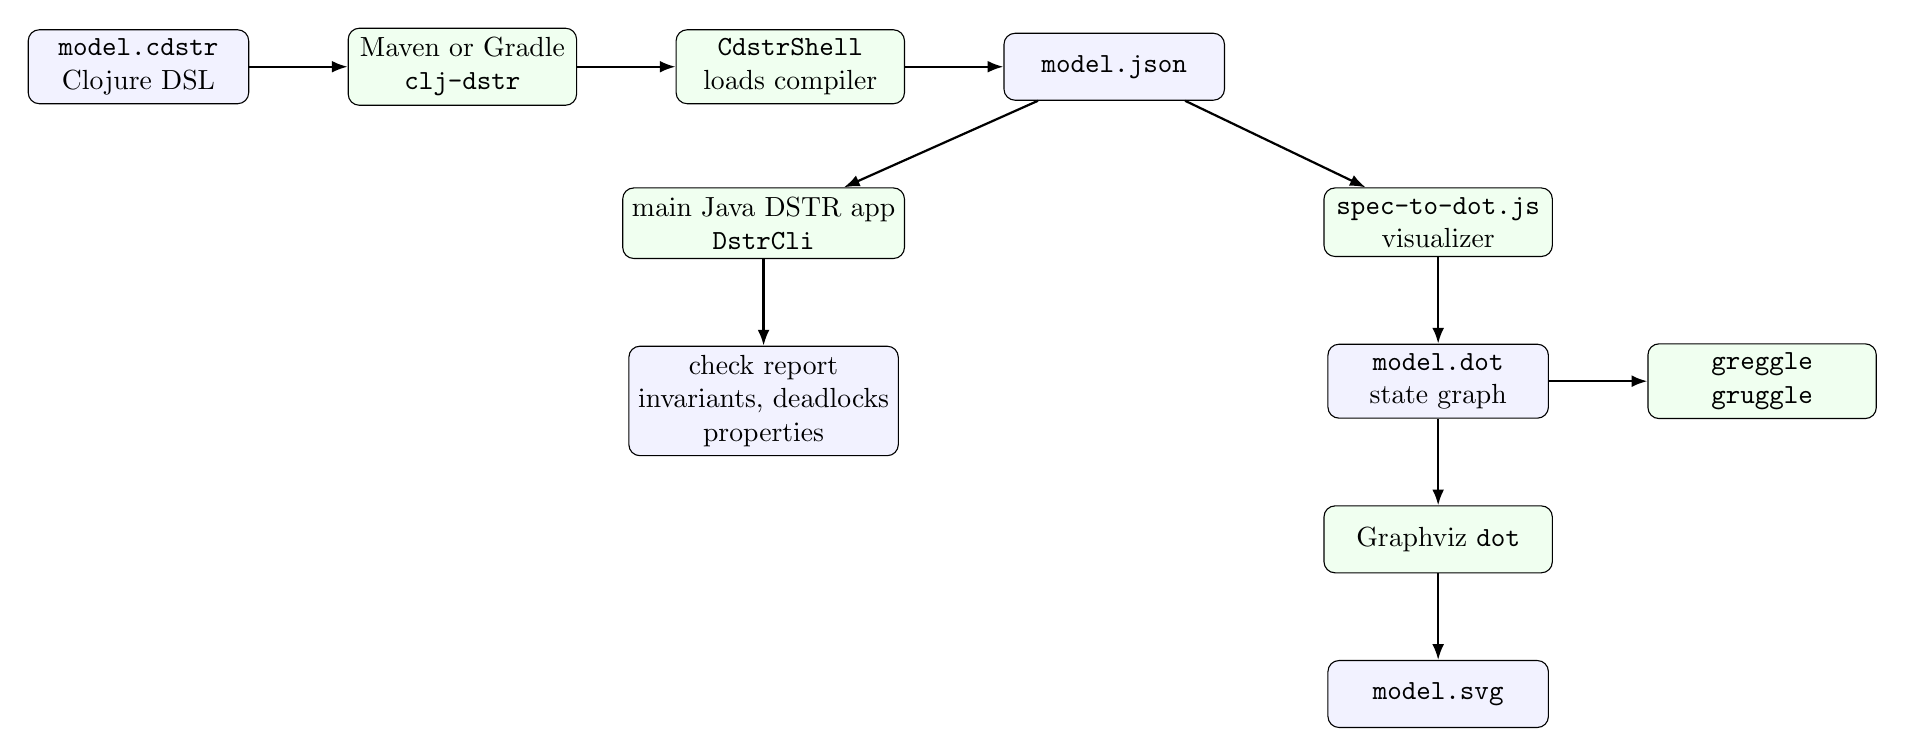
\begin{tikzpicture}[
  node distance=1.1cm and 1.25cm,
  box/.style={draw, rounded corners, align=center, minimum width=2.8cm,
    minimum height=0.85cm, fill=blue!5},
  tool/.style={draw, rounded corners, align=center, minimum width=2.9cm,
    minimum height=0.85cm, fill=green!6},
  arr/.style={-{Latex[length=2mm]}, thick}
]
\node[box] (src) {\texttt{model.cdstr}\\Clojure DSL};
\node[tool, right=of src] (mvn) {Maven or Gradle\\\texttt{clj-dstr}};
\node[tool, right=of mvn] (shell) {\texttt{CdstrShell}\\loads compiler};
\node[box, right=of shell] (json) {\texttt{model.json}};
\node[tool, below left=of json] (checker) {main Java DSTR app\\\texttt{DstrCli}};
\node[box, below=of checker] (report) {check report\\invariants, deadlocks\\properties};
\node[tool, below right=of json] (dot) {\texttt{spec-to-dot.js}\\visualizer};
\node[box, below=of dot] (dotfile) {\texttt{model.dot}\\state graph};
\node[tool, below=of dotfile] (graphviz) {Graphviz \texttt{dot}};
\node[box, below=of graphviz] (svg) {\texttt{model.svg}};
\node[tool, right=of dotfile] (gg) {\texttt{greggle}\\\texttt{gruggle}};
\draw[arr] (src) -- (mvn);
\draw[arr] (mvn) -- (shell);
\draw[arr] (shell) -- (json);
\draw[arr] (json) -- (checker);
\draw[arr] (checker) -- (report);
\draw[arr] (json) -- (dot);
\draw[arr] (dot) -- (dotfile);
\draw[arr] (dotfile) -- (graphviz);
\draw[arr] (dotfile) -- (gg);
\draw[arr] (graphviz) -- (svg);
\end{tikzpicture}
}
\end{center}

The Clojure project is only the front end: it turns \texttt{.cdstr} into the
shared JSON representation.  The main model-checking step is performed by the
root Java DSTR application, \texttt{org.dstr.cli.DstrCli}.  Use that checker
for invariant checking, deadlock detection, transition counts, and
\texttt{eventually} property results.  Use \texttt{spec-to-dot.js} and Graphviz
when you also want a visual state graph.  The generated \texttt{.dot} graph can
also serve as input to \texttt{greggle} and \texttt{gruggle} for graph
interrogation and manipulation.

\section{Command Reference}

\subsection{Repository Wrappers}

From the repository root, use \texttt{cdstr.bat} or \texttt{cdstr.sh} to compile
a single \texttt{.cdstr} file to JSON.

\begin{lstlisting}[language=bash]
.\cdstr.bat cdstr-testsuite\light-switch.cdstr
.\cdstr.bat cdstr-testsuite\light-switch.cdstr target\light-switch.json
\end{lstlisting}

\begin{lstlisting}[language=bash]
./cdstr.sh cdstr-testsuite/light-switch.cdstr
./cdstr.sh cdstr-testsuite/light-switch.cdstr target/light-switch.json
\end{lstlisting}

If the output path is omitted, the wrapper writes a JSON file adjacent to the
source file.

\subsection{SVG Wrapper}

\begin{lstlisting}[language=bash]
.\cdstr-to-svg.bat cdstr-testsuite\light-switch.cdstr
.\cdstr-to-svg.bat cdstr-testsuite\bakery-3proc.cdstr --max-states 500
\end{lstlisting}

\begin{lstlisting}[language=bash]
./cdstr-to-svg.sh cdstr-testsuite/light-switch.cdstr
./cdstr-to-svg.sh cdstr-testsuite/bakery-3proc.cdstr --max-states 500
\end{lstlisting}

The SVG wrapper accepts \texttt{input.cdstr} or \texttt{input.json}.  For source
input it produces adjacent \texttt{.json}, \texttt{.dot}, and \texttt{.svg}
files.  For JSON input it reuses the normalized spec directly.  This wrapper is
for visualization; run the Java model checker when the goal is a checking
report.  Use the \texttt{.svg} output for viewing and the \texttt{.dot} output
as input to \texttt{greggle} or \texttt{gruggle}.

\subsection{Run the Java Model Checker}

After producing JSON with \texttt{cdstr}, run the root Java DSTR application:

\begin{lstlisting}[language=bash]
mvn exec:java -Dexec.args="cdstr-testsuite/light-switch.json"
gradle run --args="cdstr-testsuite/light-switch.json"
\end{lstlisting}

The checker enumerates the finite state space, starts from all states
satisfying \texttt{init}, follows the \texttt{next} relation, checks invariants
on reachable states, records deadlock paths, and reports existential
reachability results for \texttt{eventually} properties.  Its output is the
authoritative check result for the normalized JSON produced by CDSTR.

\subsection{Running the Standalone Project}

The Clojure front end can also be run from inside \texttt{clj-dstr}.

\begin{lstlisting}[language=bash]
cd clj-dstr
mvn compile exec:java -Dexec.args="samples/light-switch.cdstr target/light-switch.json"
\end{lstlisting}

\begin{lstlisting}[language=bash]
cd clj-dstr
gradle run --args="samples/light-switch.cdstr target/light-switch.json"
\end{lstlisting}

Directory inputs are accepted:

\begin{lstlisting}[language=bash]
mvn -q -f clj-dstr/pom.xml compile exec:java \
  "-Dexec.args=cdstr-testsuite target/cdstr-generated"
\end{lstlisting}

\section{Reader Model}

CDSTR source is read by the Clojure reader.  That has several practical
consequences:

\begin{itemize}
\item Parenthesized forms are ordinary Clojure lists.
\item Clojure \texttt{defn} and \texttt{defmacro} can appear before the
  \texttt{system} form.
\item \texttt{include}, \texttt{load-java-enums}, and
  \texttt{load-proto-enums} can also appear before \texttt{system}; relative
  paths are resolved from the current CDSTR file.
\item Clojure comments beginning with \texttt{;} are available.
\item Symbols such as \texttt{light+} and \texttt{\$turn-on} are legal Clojure
  symbols and are interpreted by the CDSTR compiler.
\item The reader macro \texttt{@x} means Clojure dereference.  Prefer
  \texttt{\$action} or \texttt{(action-ref action)} for action references.
\end{itemize}

\section{System Form}

\begin{lstlisting}[language=CDSTR]
(system light-switch
  (vars light)
  (domain light off on)
  (init (= light off))
  (action turn-on
    (= light off)
    (= light+ on))
  (action turn-off
    (= light on)
    (= light+ off))
  (next (or $turn-on $turn-off))
  (invariant type-ok
    (in light (set off on)))
  (property eventually-on
    (eventually (= light on))))
\end{lstlisting}

The top-level system clauses are:

\begin{description}
\item[\texttt{vars}] Declare state variables.
\item[\texttt{vars*}] Declare a Cartesian product of variable names.
\item[\texttt{domain}] Declare one finite domain.  A single
  \texttt{\$EnumName} value expands to the symbols loaded from a Java enum type.
\item[\texttt{domain*}] Declare domains for variables matching a glob pattern.
\item[\texttt{init}] Define initial-state predicate.
\item[\texttt{action}] Define a named transition predicate.
\item[\texttt{next}] Define the next-state relation.
\item[\texttt{invariant}] Define a predicate checked on reachable states.
\item[\texttt{property}] Define a property summary, commonly with
  \texttt{eventually}.
\end{description}

Multiple body forms in a clause are compiled as an implicit conjunction.

\section{Atoms and References}

\begin{description}
\item[Current variable] A declared symbol such as \texttt{pc}.
\item[Next variable] A declared symbol with \texttt{+}, such as \texttt{pc+}.
\item[Action reference] \texttt{\$p1-start}, \texttt{(action-ref p1-start)}, or
  Clojure's dereference form if it reaches the compiler as \texttt{(deref
  p1-start)}.  New CDSTR models should use \texttt{\$action}.
\item[Domain literal] An undeclared symbol in a domain body becomes a string
  literal.
\item[Expression literal] An undeclared symbol in expressions also becomes a
  string literal unless it is a local quantified variable.
\item[Booleans] Clojure \texttt{true}, \texttt{false}, and \texttt{nil} are
  accepted; \texttt{t} is also accepted as true for lispy parity.
\item[Numbers and strings] Clojure numbers and strings become JSON numeric and
  string literals.
\end{description}

\section{Expression Reference}

\subsection{Logic}

\begin{lstlisting}[language=CDSTR]
(and (= pc idle) (= lock free))
(or $enter $exit)
(not (= pc cs))
(implies (= pc cs) (= lock held))
\end{lstlisting}

\subsection{Comparison and Arithmetic}

\begin{lstlisting}[language=CDSTR]
(= hr 12)
(!= mem 0)
(< ticket other-ticket)
(= hr+ (if-wrap (+ hr 1))) ; user macro/function may produce DSL
(= next-count (+ count 1))
\end{lstlisting}

The DSL operators include \texttt{=}, \texttt{!=}, \texttt{<}, \texttt{<=},
\texttt{>}, \texttt{>=}, \texttt{+}, \texttt{-}, \texttt{*}, and \texttt{/}.

\subsection{Sets}

\begin{lstlisting}[language=CDSTR]
(domain mode idle running stopped)
(in mode (set idle running stopped))
(= allowed (set p1 p2 p3))
\end{lstlisting}

\subsection{Domains from Java Enums}

\texttt{load-java-enums} accepts one or more Java files or directories before
the \texttt{system} form.  Directories are searched recursively.  The enum
scanner is lightweight and intended for conventional declarations with
comma-separated constants, including comments and whitespace.

\begin{lstlisting}[language=CDSTR]
(load-java-enums "src/main/java")

(system lifecycle-model
  (vars state)
  (domain state $Lifecycle)
  (init (= state "NEW"))
  (action activate
    (= state "NEW")
    (set state as "READY"))
  (next $activate))
\end{lstlisting}

CDSTR preserves Clojure string literals exactly, so the Java constants
\texttt{NEW} and \texttt{READY} are shown as upper-case strings here.

\subsection{Domains from Protocol Buffer Enums}

\texttt{load-proto-enums} accepts one or more \texttt{.proto} files or
directories before the \texttt{system} form.  Directories are searched
recursively.  The parser recognizes entries of the form \texttt{NAME = number;}
and ignores comments, enum options, reserved declarations, and option values.

\begin{lstlisting}[language=CDSTR]
(load-proto-enums "src/main/proto")

(system order-model
  (vars status)
  (domain status $OrderStatus)
  (init (= status ORDER_STATUS_NEW))
  (action ready
    (= status ORDER_STATUS_NEW)
    (set status as ORDER_STATUS_READY))
  (next $ready))
\end{lstlisting}

CDSTR preserves the protobuf enum symbol spelling shown in the source file.

\subsection{Quantifiers}

\begin{lstlisting}[language=CDSTR]
(forall (p in (set p1 p2))
  (in p (set p1 p2)))

(exists (candidate in (set p1 p2))
  (= candidate owner))
\end{lstlisting}

\subsection{Reachability-Style Properties}

\begin{lstlisting}[language=CDSTR]
(property can-measure-four-gallons
  (eventually (= big 4)))
\end{lstlisting}

\texttt{eventually} is interpreted by the prototype as ``some reachable state
satisfies this predicate.''

\section{Transition Sugar}

\subsection{Assignment}

All three forms assert equality between the next state of a variable and a
value:

\begin{lstlisting}[language=CDSTR]
(= light+ on)
(assign on to light)
(set light as on)
\end{lstlisting}

\subsection{Unconditional Transitions}

An action body is a conjunction of its forms.  For an unconditional transition,
write the next-state assignments directly:

\begin{lstlisting}[language=CDSTR]
(action reset
  (assign IDLE to pc)
  (set count as 0)
  (assign false to busy))
\end{lstlisting}

The same transition can be written with explicit next-state equalities:

\begin{lstlisting}[language=CDSTR]
(action reset
  (= pc+ IDLE)
  (= count+ 0)
  (= busy+ false))
\end{lstlisting}

Frame variables that should not change:

\begin{lstlisting}[language=CDSTR]
(action reset
  (assign IDLE to pc)
  (set count as 0)
  (unchanged owner mode))
\end{lstlisting}

or use glob-based frame sugar:

\begin{lstlisting}[language=CDSTR]
(action reset
  (assign IDLE to pc)
  (set count as 0)
  (unchanged* *_status *_version))
\end{lstlisting}

If an action does not constrain a next-state variable, the checker may consider
all values in that variable's domain as possible successor values.

\subsection{Equality Alias}

\begin{lstlisting}[language=CDSTR]
(equals master_lifecycle ENRICHING)
\end{lstlisting}

is equivalent to:

\begin{lstlisting}[language=CDSTR]
(= master_lifecycle ENRICHING)
\end{lstlisting}

\subsection{Guarded Cases}

\begin{lstlisting}[language=CDSTR]
(if
  (equals master_lifecycle ENRICHING)
  (equals venue1_lifecycle ENRICHING)
  then
  (assign READY to master_lifecycle)
  (assign READY to venue1_lifecycle)
  (assign NOT_TRADING to master_trading_status)
  (assign NOT_TRADING to venue1_trading_status))
\end{lstlisting}

The CDSTR compiler accepts multiple condition forms before \texttt{then} and
multiple consequence forms after \texttt{then}.  The result is a conjunction of
all condition and consequence forms.  There is no \texttt{else} branch.

\subsection{Frame Conditions}

\begin{lstlisting}[language=CDSTR]
(unchanged* *_market_status *_event_type *_mission_version)
\end{lstlisting}

This emits frame equalities for every declared variable matched by the glob
patterns.

\subsection{Scenario Alias}

\begin{lstlisting}[language=CDSTR]
(alternate-scenarios
  (if (= state OPEN) then (assign CANCELLED to state))
  (if (= state BOOKED) then (assign state to state)))
\end{lstlisting}

\texttt{alternate-scenarios} is a synonym for \texttt{or}.

\section{Clojure Macros}

The \texttt{system} macro captures the unevaluated DSL body, then the compiler
macroexpands recognized non-reserved Clojure macro calls before normalizing the
model.  A macro can return one DSL form or a sequence of sibling forms.

\subsection{Built-In Helpers}

\begin{lstlisting}[language=CDSTR]
(same pc)                 ; expands to (= pc+ pc)
(unchanged p2pc mem)      ; expands to sibling frame clauses
(next-var-symbol 'pc)     ; returns symbol pc+
\end{lstlisting}

\subsection{Simple Clojure Macro}

\begin{lstlisting}[language=CDSTR]
(defmacro preserve [& vars]
  (mapv (fn [v] (list '= (next-var-symbol v) v)) vars))

(system example
  (vars pc mem)
  (domain pc idle done)
  (domain mem 0 1)
  (init (= pc idle) (= mem 0))
  (action finish
    (= pc idle)
    (= pc+ done)
    (preserve mem))
  (next $finish))
\end{lstlisting}

Here \texttt{preserve} returns sibling frame clauses.  The compiler splices
those clauses into the containing action body.

\subsection{Including Helper Files}

\begin{lstlisting}[language=CDSTR]
(include "helpers.clj")

(system uses-helper
  ...)
\end{lstlisting}

Relative include paths are resolved against the directory of the current
\texttt{.cdstr} file.  The Java and proto enum loaders use the same
relative-path rule.

\section{Product Variables and Large Models}

\begin{lstlisting}[language=CDSTR]
(system trade-cancellation-parent-children-small
  (vars* _ (p c1 c2) * (market_status settlement_state settlement_version settlement_revision event_type))

  (domain* *_market_status MATCHED)
  (domain* *_settlement_state OPEN RELEASED BOOKED CANCELLED)
  (domain* *_event_type INSTRUCTION_ACKED)
  (domain* *_mission_version 1)
  (domain* *_mission_revision 1)

  (init
    (equals p_settlement_state OPEN)
    (equals c1_settlement_state OPEN)
    (equals c2_settlement_state OPEN))

  (action trade-cancellation
    (unchanged* *_market_status *_event_type *_mission_version *_mission_revision)
    (alternate-scenarios
      (if
        (equals p_settlement_state OPEN)
        (equals c1_settlement_state OPEN)
        (equals c2_settlement_state OPEN)
        then
        (assign CANCELLED to p_settlement_state)
        (assign CANCELLED to c1_settlement_state)
        (assign CANCELLED to c2_settlement_state))))

  (next $trade-cancellation))
\end{lstlisting}

Use \texttt{--max-states} when visualizing large explicit-domain variants.

\section{State Graph Interpretation}

\begin{center}
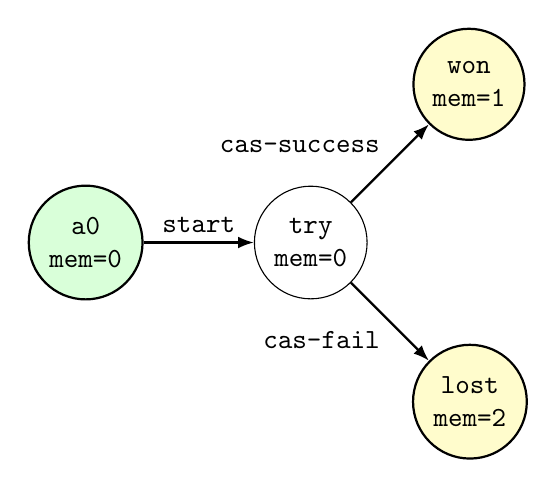
\begin{tikzpicture}[
  node distance=1.4cm,
  state/.style={circle, draw, minimum size=1cm, align=center},
  init/.style={state, fill=green!15, thick},
  dead/.style={state, fill=yellow!20, thick},
  arr/.style={-{Latex[length=2mm]}, thick}
]
\node[init] (a0) {\texttt{a0}\\\texttt{mem=0}};
\node[state, right=of a0] (try) {\texttt{try}\\\texttt{mem=0}};
\node[dead, above right=of try] (won) {\texttt{won}\\\texttt{mem=1}};
\node[dead, below right=of try] (lost) {\texttt{lost}\\\texttt{mem=2}};
\draw[arr] (a0) -- node[above] {\texttt{start}} (try);
\draw[arr] (try) -- node[above left] {\texttt{cas-success}} (won);
\draw[arr] (try) -- node[below left] {\texttt{cas-fail}} (lost);
\end{tikzpicture}
\end{center}

The Graphviz output labels reachable counts, visible transitions, deadlocks,
invariant failures, actions, and property truth values.  Compact graphs move
the action and property summaries into a legend node.

\section{CDSTR Test Suite}

The \texttt{cdstr-testsuite} directory mirrors the DSTR and TDSTR examples.
It includes:

\begin{itemize}
\item \texttt{light-switch.cdstr}
\item \texttt{tla-hour-clock.cdstr}
\item \texttt{tla-die-hard.cdstr}
\item \texttt{tla-peterson-2proc.cdstr}
\item \texttt{bakery-3proc.cdstr}
\item \texttt{cas-2proc-race.cdstr}
\item \texttt{instrument-lifecycle.cdstr}
\item \texttt{instrument-lifecycle-small.cdstr}
\item \texttt{trade-cancellation-parent-children.cdstr}
\item \texttt{trade-cancellation-parent-children-small.cdstr}
\end{itemize}

Compile the suite:

\begin{lstlisting}[language=bash]
mvn -q -f clj-dstr/pom.xml compile exec:java \
  "-Dexec.args=cdstr-testsuite target/cdstr-generated"
\end{lstlisting}

Then pass any generated JSON file to the root Java checker:

\begin{lstlisting}[language=bash]
mvn exec:java -Dexec.args="target/cdstr-generated/light-switch.json"
\end{lstlisting}

\section{Practical Notes}

\begin{itemize}
\item Prefer \texttt{\$action} for action references in CDSTR.  It is portable
  across the lispy front ends and avoids Clojure reader-deref ambiguity.
\item Keep user macro names distinct from reserved DSL heads such as
  \texttt{action}, \texttt{if}, \texttt{set}, and \texttt{forall}.
\item A macro that returns sibling clauses should return a sequence of forms,
  not a quoted wrapper form.
\item Next-state variables are only meaningful in transition contexts:
  \texttt{action} and \texttt{next}.
\item Clojure code runs at compile time.  Keep helper macros deterministic so
  generated JSON remains reproducible.
\item Treat CDSTR as the source-language layer and the root Java DSTR
  application as the checking layer.  The SVG tooling is for graph inspection.
\end{itemize}

\end{document}
